\newpage
\section{Projekt systemu}
\label{sec:projekt}

Projekt opisuje, jak system zrealizuje wymagania z~sekcji~\ref{sec:specyfikacja}.
Powiązanie elementów projektu z~wymaganiami zestawiono
w~podsekcji~\ref{sec:powiazanie}.

\subsection{Architektura systemu}

\begin{center}
    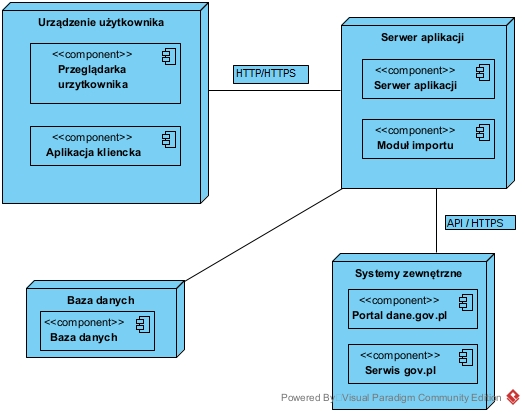
\includegraphics[width=0.75\linewidth]{Diagram_architektury_systemu}
\end{center}

System składa się z~następujących elementów:

\begin{itemize}
    \item \textbf{Przeglądarka użytkownika} -- uruchamia aplikację na
    telefonie lub komputerze (O-03). W~pamięci przeglądarki przechowywane są
    wybrana rola oraz lista ostatnio przeglądanych środków (WF-05, WF-15).
    \item \textbf{Aplikacja kliencka (frontend)} -- interfejs zaprojektowany
    w~podejściu \emph{Mobile First}. Wysyła zapytania do serwera i~prezentuje
    otrzymane wyniki.
    \item \textbf{Serwer aplikacji (API)} -- obsługuje wyszukiwanie,
    podpowiedzi, karty środków i~zamienniki. Zwraca wyłącznie dane potrzebne
    do wyświetlenia bieżącego widoku.
    \item \textbf{Baza danych} -- przechowuje dane rejestru i~historię
    wczytywania danych.
    \item \textbf{Moduł importu} -- proces uruchamiany codziennie przez
    harmonogram, niezależny od obsługi użytkowników. Pobiera nowe pliki przez
    API portalu dane.gov.pl i~wczytuje je do bazy danych.
    \item \textbf{Systemy zewnętrzne} -- portal dane.gov.pl (źródło danych,
    O-01) oraz serwis gov.pl, na którym publikowane są etykiety środków
    w~formacie PDF.
\end{itemize}

\subsubsection{Decyzje projektowe}

\begin{itemize}
    \item \textbf{Wyszukiwanie po stronie serwera.} Urządzenie użytkownika
    pobiera tylko wyniki zapytania, a~nie całą bazę środków, jak w~wyszukiwarce
    ministerstwa. Pozwala to spełnić WNF-01 i~WNF-02 również przy słabym
    zasięgu.
    \item \textbf{Brak uwierzytelniania.} System nie ma kont ani panelu
    administracyjnego (WNF-09, O-04), dlatego nie zawiera modułu logowania.
    Dane związane z~użytkownikiem pozostają na jego urządzeniu.
    \item \textbf{Wczytywanie danych w~całości albo wcale.} Moduł importu
    wczytuje nowe pliki do tabel tymczasowych, sprawdza ich poprawność,
    a~następnie w~jednej transakcji zastępuje nimi poprzednie dane. Błąd na
    dowolnym etapie pozostawia poprzednią wersję danych bez zmian (WNF-08).
    \item \textbf{Codzienne sprawdzanie publikacji.} Moduł importu porównuje
    datę publikacji plików na portalu z~datą ostatnio wczytanej wersji
    i~pobiera dane tylko wtedy, gdy pojawiła się nowa wersja. Codzienne
    sprawdzanie zapewnia spełnienie WNF-07 (najwyżej 7~dni od publikacji).
\end{itemize}

\subsubsection{Wybór technologii}

Na tym etapie wybrano wyłącznie system bazy danych, ponieważ wynika on
bezpośrednio z~charakteru danych i~wymagań. Pozostałe technologie zostaną
dobrane na etapie implementacji.

Wybrano bazę danych \textbf{PostgreSQL}, ponieważ:

\begin{itemize}
    \item dane rejestru mają charakter relacyjny -- środki, substancje czynne,
    zastosowania, uprawy i~agrofagi są ze sobą powiązane relacjami
    wiele-do-wielu, a~filtrowanie krzyżowe (WF-04) sprowadza się do złączeń
    tabel,
    \item standardowe rozszerzenia PostgreSQL realizują wyszukiwanie odporne
    na literówki (WF-02) bez osobnego silnika wyszukiwania: \emph{pg\_trgm}
    (indeks trigramowy, szybkie wyszukanie podobnych nazw),
    \emph{fuzzystrmatch} (odległość edycyjna, czyli sprawdzenie warunku
    ,,najwyżej 2~znaki'') oraz \emph{unaccent} (porównywanie nazw bez względu
    na polskie znaki),
    \item transakcje obejmujące wiele tabel pozwalają zrealizować podmianę
    danych w~całości albo wcale (WNF-08).
\end{itemize}

\subsection{Moduły systemu}

\begingroup
\small
\begin{longtable}{|>{\raggedright\arraybackslash}p{3cm}|p{9.4cm}|>{\raggedright\arraybackslash}p{2.2cm}|}
\hline
\textbf{Moduł} & \textbf{Odpowiedzialność} & \textbf{Wymagania} \\
\hline
\endfirsthead
\hline
\textbf{Moduł} & \textbf{Odpowiedzialność} & \textbf{Wymagania} \\
\hline
\endhead
Wyszukiwanie &
Wyszukiwanie środków po nazwie handlowej i~substancji czynnej z~tolerancją
literówek, filtrowanie krzyżowe po uprawie, agrofagu i~rodzaju środka,
ograniczenie wyników do wybranej roli, informacja o~środkach usuniętych
z~rejestru. &
WF-01 -- WF-05, WF-12 \\
\hline
Podpowiedzi słownikowe &
Podpowiadanie nazw upraw, agrofagów, substancji czynnych i~rodzajów środków
podczas wpisywania, z~tolerancją literówek. Wybrana pozycja jest przekazywana
do wyszukiwania jako jednoznaczny identyfikator. &
WF-02 -- WF-04 \\
\hline
Karta środka &
Prezentacja danych środka i~wszystkich jego zastosowań, okresu karencji lub
odnośnika do etykiety, oznaczenia upływającego terminu dopuszczenia oraz
stałego adresu karty. &
WF-06, WF-07, WF-08, WF-11, WF-16 \\
\hline
Zamienniki &
Wyszukiwanie środków o~tych samych substancjach czynnych, sortowanie według
zgodności zawartości, filtrowanie według uprawy i~roli, pomijanie środków,
których termin dopuszczenia do stosowania upłynął. &
WF-05, WF-10 \\
\hline
Etykiety &
Wyświetlanie etykiety w~aplikacji i~jej pobieranie na urządzenie. &
WF-09 \\
\hline
Import danych &
Sprawdzanie publikacji na portalu, pobieranie plików, kontrola ich
poprawności, ujednolicanie nazw, wczytanie i~podmiana danych, zapis
przebiegu i~błędów w~dzienniku zdarzeń. &
WF-13, WF-14, WNF-07, WNF-08 \\
\hline
Preferencje lokalne &
Zapamiętywanie roli i~listy 10 ostatnio przeglądanych środków w~pamięci
przeglądarki (część aplikacji klienckiej). &
WF-05, WF-15 \\
\hline
\end{longtable}
\endgroup

\subsection{Aktorzy i~przypadki użycia}

\begin{itemize}
    \item \textbf{Użytkownik} -- osoba korzystająca z~aplikacji bez konta.
    Występuje w~jednej z~dwóch ról: \textbf{użytkownik profesjonalny} lub
    \textbf{użytkownik nieprofesjonalny}. Obie role mają te same przypadki
    użycia, a~rola wpływa jedynie na zakres prezentowanych środków.
    \item \textbf{Harmonogram} -- aktor systemowy, który codziennie uruchamia
    aktualizację danych.
    \item \textbf{Portal dane.gov.pl} -- system zewnętrzny udostępniający
    pliki rejestru.
\end{itemize}

\begingroup
\small
\begin{longtable}{|p{1.3cm}|>{\raggedright\arraybackslash}p{6.1cm}|>{\raggedright\arraybackslash}p{3cm}|>{\raggedright\arraybackslash}p{3.7cm}|}
\hline
\textbf{ID} & \textbf{Przypadek użycia} & \textbf{Aktor} & \textbf{Wymagania} \\
\hline
\endfirsthead
\hline
\textbf{ID} & \textbf{Przypadek użycia} & \textbf{Aktor} & \textbf{Wymagania} \\
\hline
\endhead
PU-01 & Wyszukaj środek po nazwie & Użytkownik & WF-01, WF-02, WF-12 \\
\hline
PU-02 & Wyszukaj środki po substancji czynnej & Użytkownik & WF-02, WF-03 \\
\hline
PU-03 & Znajdź środek na agrofaga w~uprawie & Użytkownik & WF-02, WF-04, WF-05 \\
\hline
PU-04 & Wybierz rolę & Użytkownik & WF-05 \\
\hline
PU-05 & Przeglądaj kartę środka & Użytkownik & WF-06, WF-07, WF-08, WF-11 \\
\hline
PU-06 & Wyświetl lub pobierz etykietę & Użytkownik & WF-09 \\
\hline
PU-07 & Znajdź zamienniki środka & Użytkownik & WF-05, WF-10 \\
\hline
PU-08 & Przeglądaj ostatnio oglądane środki & Użytkownik & WF-15 \\
\hline
PU-09 & Udostępnij kartę środka & Użytkownik & WF-16 \\
\hline
PU-10 & Zaktualizuj dane z~rejestru & Harmonogram, portal dane.gov.pl &
WF-13, WF-14, WNF-07, WNF-08 \\
\hline
\end{longtable}
\endgroup

\begin{center}
    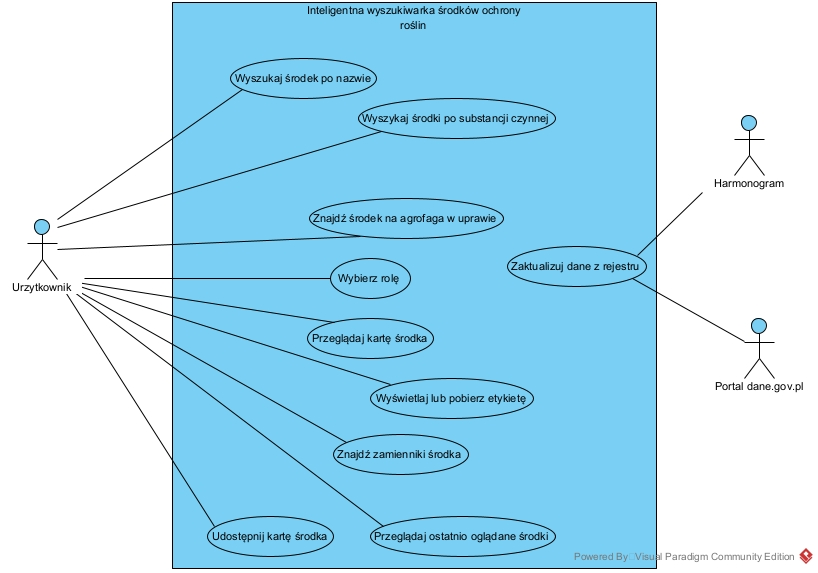
\includegraphics[width=\linewidth]{diagram_przypadkow_uzycia}
\end{center}

\subsection{Scenariusz: znalezienie środka na agrofaga w~uprawie}

Jako najważniejszą operację wybrano przypadek PU-03, ponieważ odpowiada on na
podstawowe pytanie wszystkich grup użytkowników: czym można zwalczać danego
agrofaga w~danej uprawie.

\textbf{Aktor:} użytkownik (profesjonalny lub nieprofesjonalny).

\textbf{Warunki początkowe:} w~systemie jest wczytana co najmniej jedna wersja
danych rejestru, a~użytkownik ma wybraną rolę (PU-04). Przy pierwszym
uruchomieniu aplikacja prosi o~jej wybór.

\textbf{Scenariusz główny:}

\begin{enumerate}
    \item Użytkownik otwiera wyszukiwarkę. System wyświetla formularz
    wyszukiwania, wybraną rolę oraz datę publikacji wersji danych (WF-14).
    \item Użytkownik wpisuje co najmniej 3 znaki nazwy uprawy, np.
    ,,ziemn''.
    \item System podpowiada pasujące uprawy ze słownika, również wtedy, gdy
    wpisana nazwa zawiera literówkę (WF-02).
    \item Użytkownik wybiera uprawę ,,ziemniak''. Kroki 2--4 powtarza dla
    agrofaga (,,stonka ziemniaczana'') i~opcjonalnie dla rodzaju środka.
    \item Aplikacja wysyła do serwera identyfikatory wybranych pozycji oraz
    rolę użytkownika.
    \item Serwer wybiera zastosowania spełniające wszystkie kryteria
    i~zwraca listę, w~której każdy środek występuje jeden raz (WF-04).
    W~roli nieprofesjonalnej lista obejmuje wyłącznie środki dopuszczone dla
    użytkowników nieprofesjonalnych (WF-05).
    \item System wyświetla listę środków z~nazwą, substancjami czynnymi,
    rodzajem środka i~oznaczeniem upływającego terminu dopuszczenia (WF-11).
    \item Użytkownik wybiera środek, a~system wyświetla jego kartę (PU-05).
\end{enumerate}

\textbf{Warunek końcowy:} użytkownik widzi kartę środka dopuszczonego do
zwalczania wybranego agrofaga w~wybranej uprawie.

\textbf{Scenariusze alternatywne i~sytuacje błędne:}

\begin{itemize}
    \item \textbf{3a. Brak pasującej nazwy w~słowniku.} Wpisana nazwa różni
    się od wszystkich nazw w~słowniku o~więcej niż 2 znaki. System informuje,
    że nie znaleziono takiej uprawy (lub agrofaga), a~użytkownik poprawia nazwę --
    powrót do kroku 2.
    \item \textbf{5a. Brak połączenia z~serwerem.} Aplikacja wyświetla
    komunikat o~braku połączenia, zachowuje wybrane filtry i~udostępnia
    przycisk ponowienia zapytania.
    \item \textbf{6a. Brak środków spełniających wszystkie kryteria.} System
    wyświetla komunikat o~braku wyników i~listę wybranych filtrów, z~których
    każdy można usunąć jednym dotknięciem (kryterium akceptacji WF-04).
    \item \textbf{6b. Brak środków dla roli nieprofesjonalnej.} Kryteria
    spełniają wyłącznie środki dla użytkowników profesjonalnych. System
    informuje, że dla tej uprawy i~agrofaga nie ma środków dopuszczonych dla
    użytkowników nieprofesjonalnych.
    \item \textbf{6c. Trwa lub nie powiodła się aktualizacja danych.}
    Zapytanie jest obsługiwane na poprzedniej wersji danych (WNF-08),
    a~na ekranie widnieje data jej publikacji (WF-14).
\end{itemize}

\subsection{Model danych}

\begin{center}
    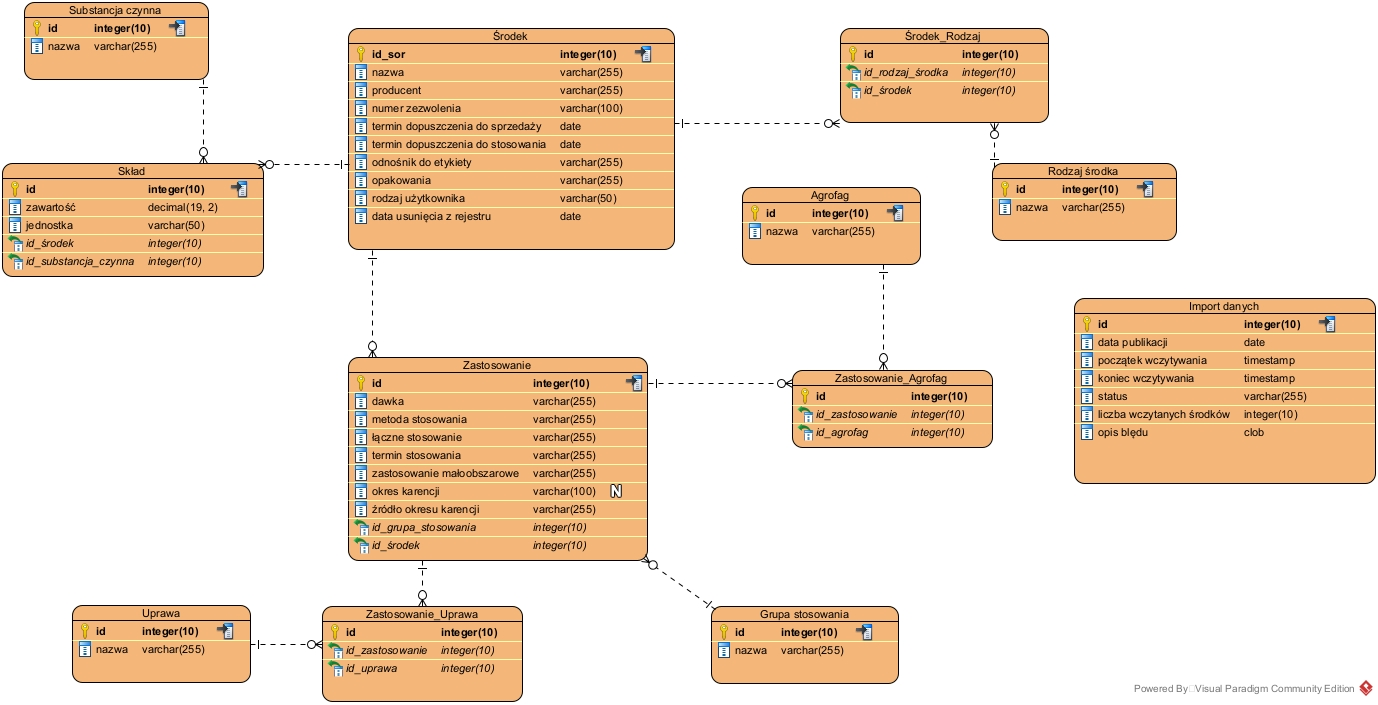
\includegraphics[width=\linewidth]{Diagram_erd}
\end{center}

Model danych odwzorowuje pliki rejestru publikowane na portalu dane.gov.pl:
rejestr podstawowy, rejestr zastosowań, rejestr kart środków, słowniki oraz
wykaz środków usuniętych z~rejestru.

\subsubsection{Decyzje dotyczące modelu}

\begin{itemize}
    \item \textbf{Jedno zastosowanie odpowiada jednemu wierszowi rejestru
    zastosowań.} Wiersz rejestru wymienia często kilka upraw i~kilkanaście
    agrofagów o~wspólnej dawce i~terminie, dlatego uprawy i~agrofagi są
    powiązane z~zastosowaniem relacjami wiele-do-wielu. Rozpisanie każdej pary
    uprawa--agrofag jako osobnego zastosowania zwiększyłoby liczbę rekordów
    z~ok.~18\,700 do ponad 158\,000.
    \item \textbf{Zastosowanie może nie mieć agrofaga.} W~rejestrze występują
    zastosowania bez wskazanego agrofaga, np. regulatorów wzrostu. Wymaganie
    agrofaga spowodowałoby pominięcie takich środków w~wynikach wyszukiwania po
    uprawie.
    \item \textbf{Zawartość substancji czynnej jako liczba z~jednostką.}
    Rejestr podaje skład w~postaci tekstu (np. ,,azoksystrobina -- 250~g'').
    Zapis liczbowy pozwala ustawić zamienniki o~tej samej zawartości na
    początku listy (WF-10).
    \item \textbf{Okres karencji jako pole opcjonalne.} Okres karencji jest
    podany tylko w~części opisów terminu stosowania (O-01). Puste pole oznacza,
    że karta środka kieruje do etykiety (WF-07), a~źródło okresu karencji
    pozwala w~przyszłości uzupełnić go danymi z~etykiet (WF-08).
    \item \textbf{Data usunięcia zamiast usuwania rekordu.} Środek usunięty
    z~rejestru pozostaje w~bazie z~datą usunięcia, dzięki czemu jego wyszukanie
    zwraca informację o~usunięciu (WF-12).
    \item \textbf{Indeksy trigramowe} na nazwach środków, substancji czynnych,
    upraw i~agrofagów przyspieszają wyszukiwanie z~tolerancją literówek
    (WF-02, WNF-01).
    \item \textbf{Dane użytkownika poza bazą.} Rola i~ostatnio przeglądane
    środki są zapisywane wyłącznie w~przeglądarce, dlatego nie występują
    w~modelu danych (WNF-09).
\end{itemize}

\subsection{Projekt najważniejszych ekranów}

Wszystkie ekrany projektowane są najpierw dla telefonu o~szerokości 360
pikseli (WNF-03), z~elementami dotykowymi o~wymiarach co najmniej
$48 \times 48$ pikseli (WNF-04), kontrastem co najmniej 7:1 (WNF-05)
i~nazewnictwem zgodnym z~rejestrem (WNF-10).

\subsubsection{E-1: Wyszukiwarka}

\begin{center}
    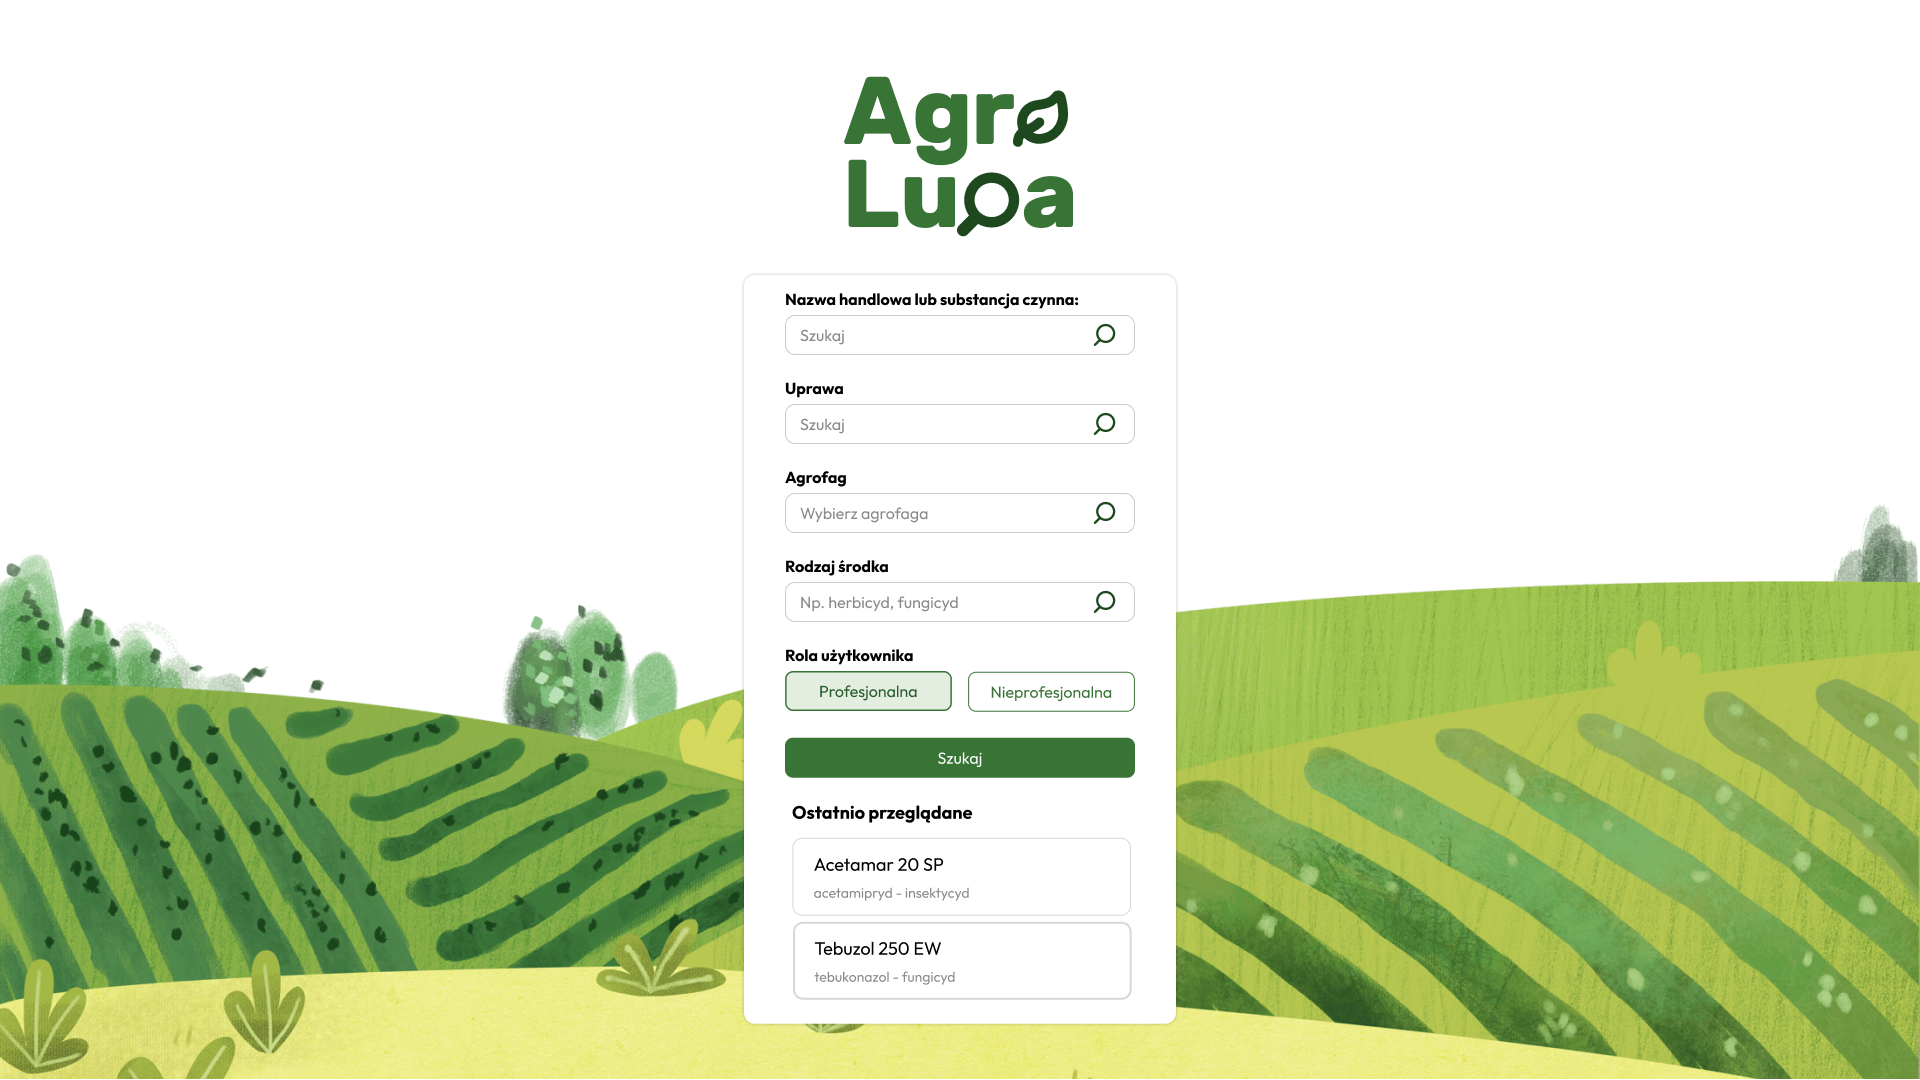
\includegraphics[width=\linewidth]{E-1_Wyszukiwarka}
\end{center}

\begin{itemize}
    \item pole wyszukiwania nazwy handlowej lub substancji czynnej,
    \item pola uprawy, agrofaga i~rodzaju środka z~podpowiedziami; wybrane
    pozycje wyświetlane są jako etykiety z~przyciskiem usunięcia,
    \item przełącznik roli: profesjonalna / nieprofesjonalna,
    \item lista ostatnio przeglądanych środków (WF-15),
    \item data publikacji wersji danych (WF-14).
\end{itemize}

\subsubsection{E-2: Lista wyników}

\begin{center}
    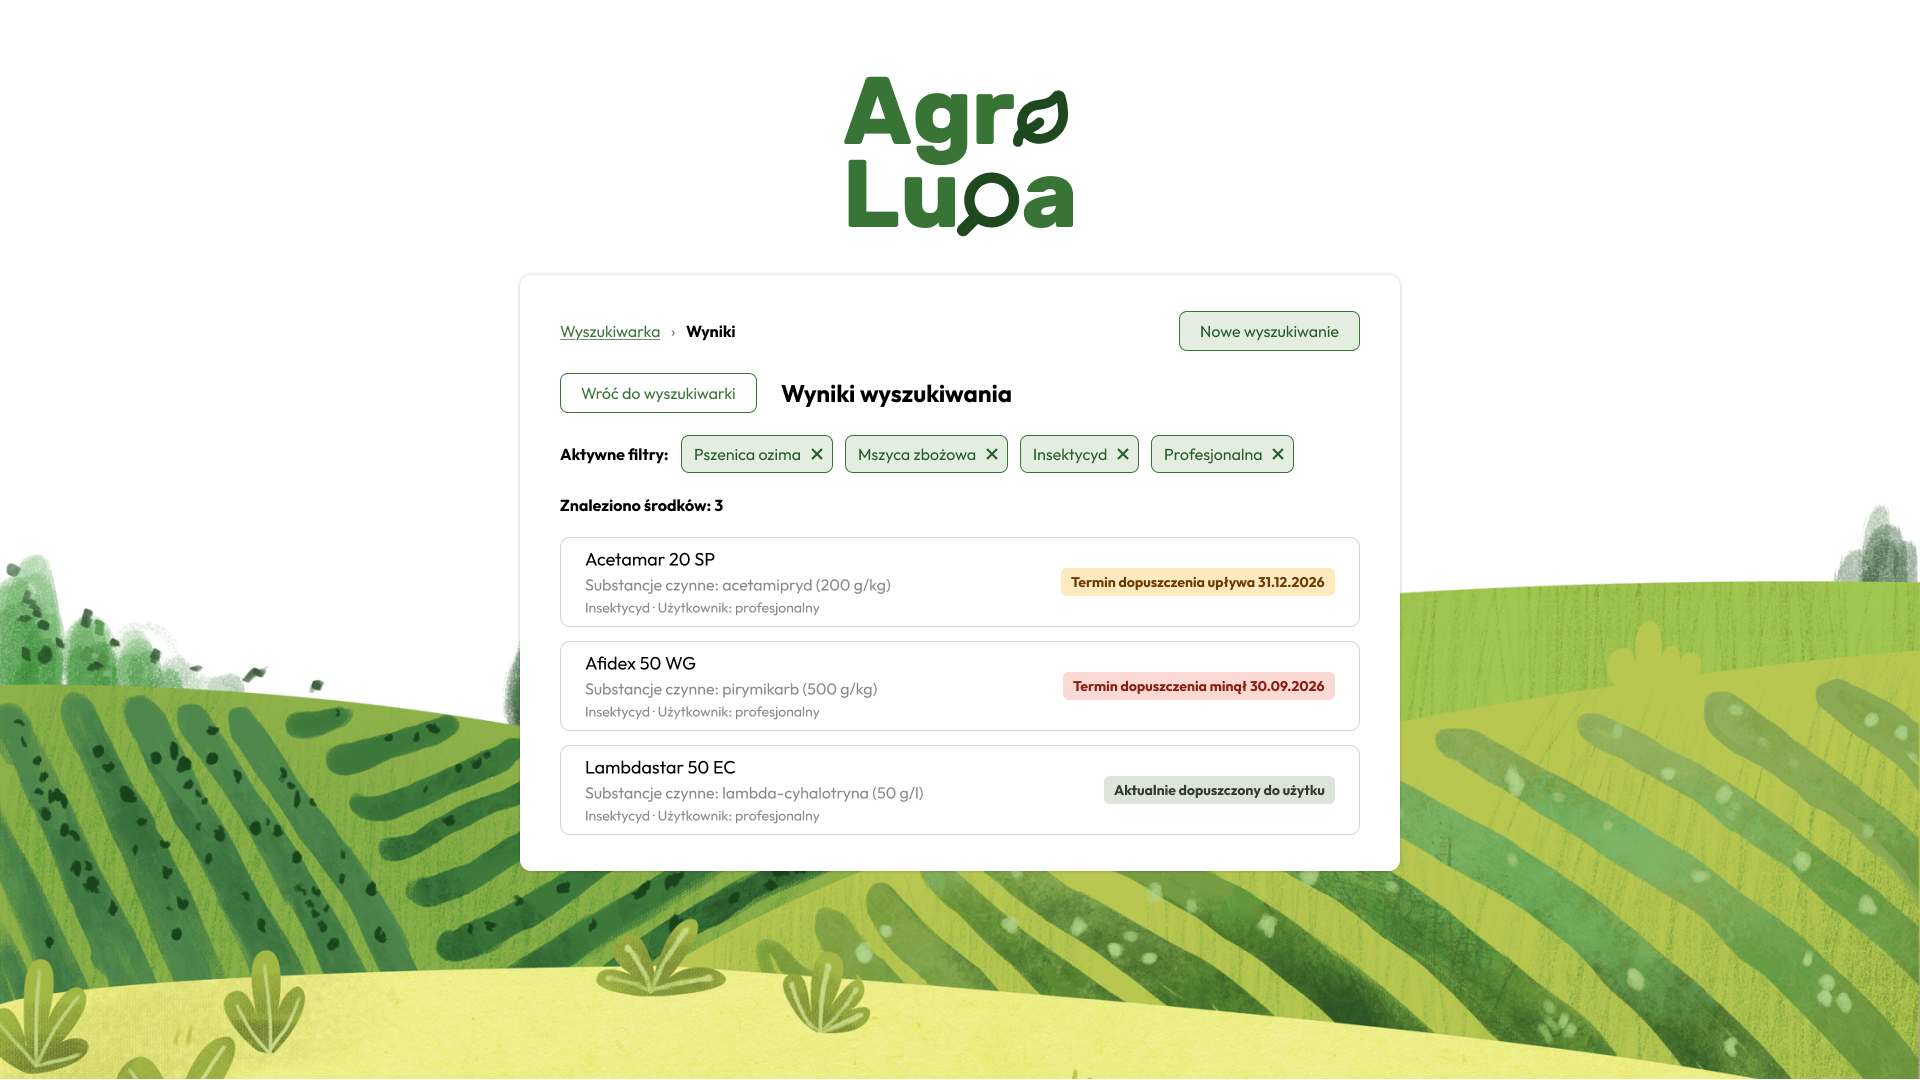
\includegraphics[width=\linewidth]{E-2_Lista_wynikow}
\end{center}

\begin{itemize}
    \item aktywne filtry z~możliwością usunięcia każdego z~nich,
    \item liczba znalezionych środków,
    \item dla każdego środka: nazwa, substancje czynne, rodzaj środka, rodzaj
    użytkownika oraz oznaczenie upływającego lub minionego terminu
    dopuszczenia (WF-11),
    \item komunikaty: brak wyników, brak środków dla roli nieprofesjonalnej,
    środek usunięty z~rejestru wraz z~datą (WF-12).
\end{itemize}

Ekran E-2 w~przypadku braku wyników:

\begin{center}
    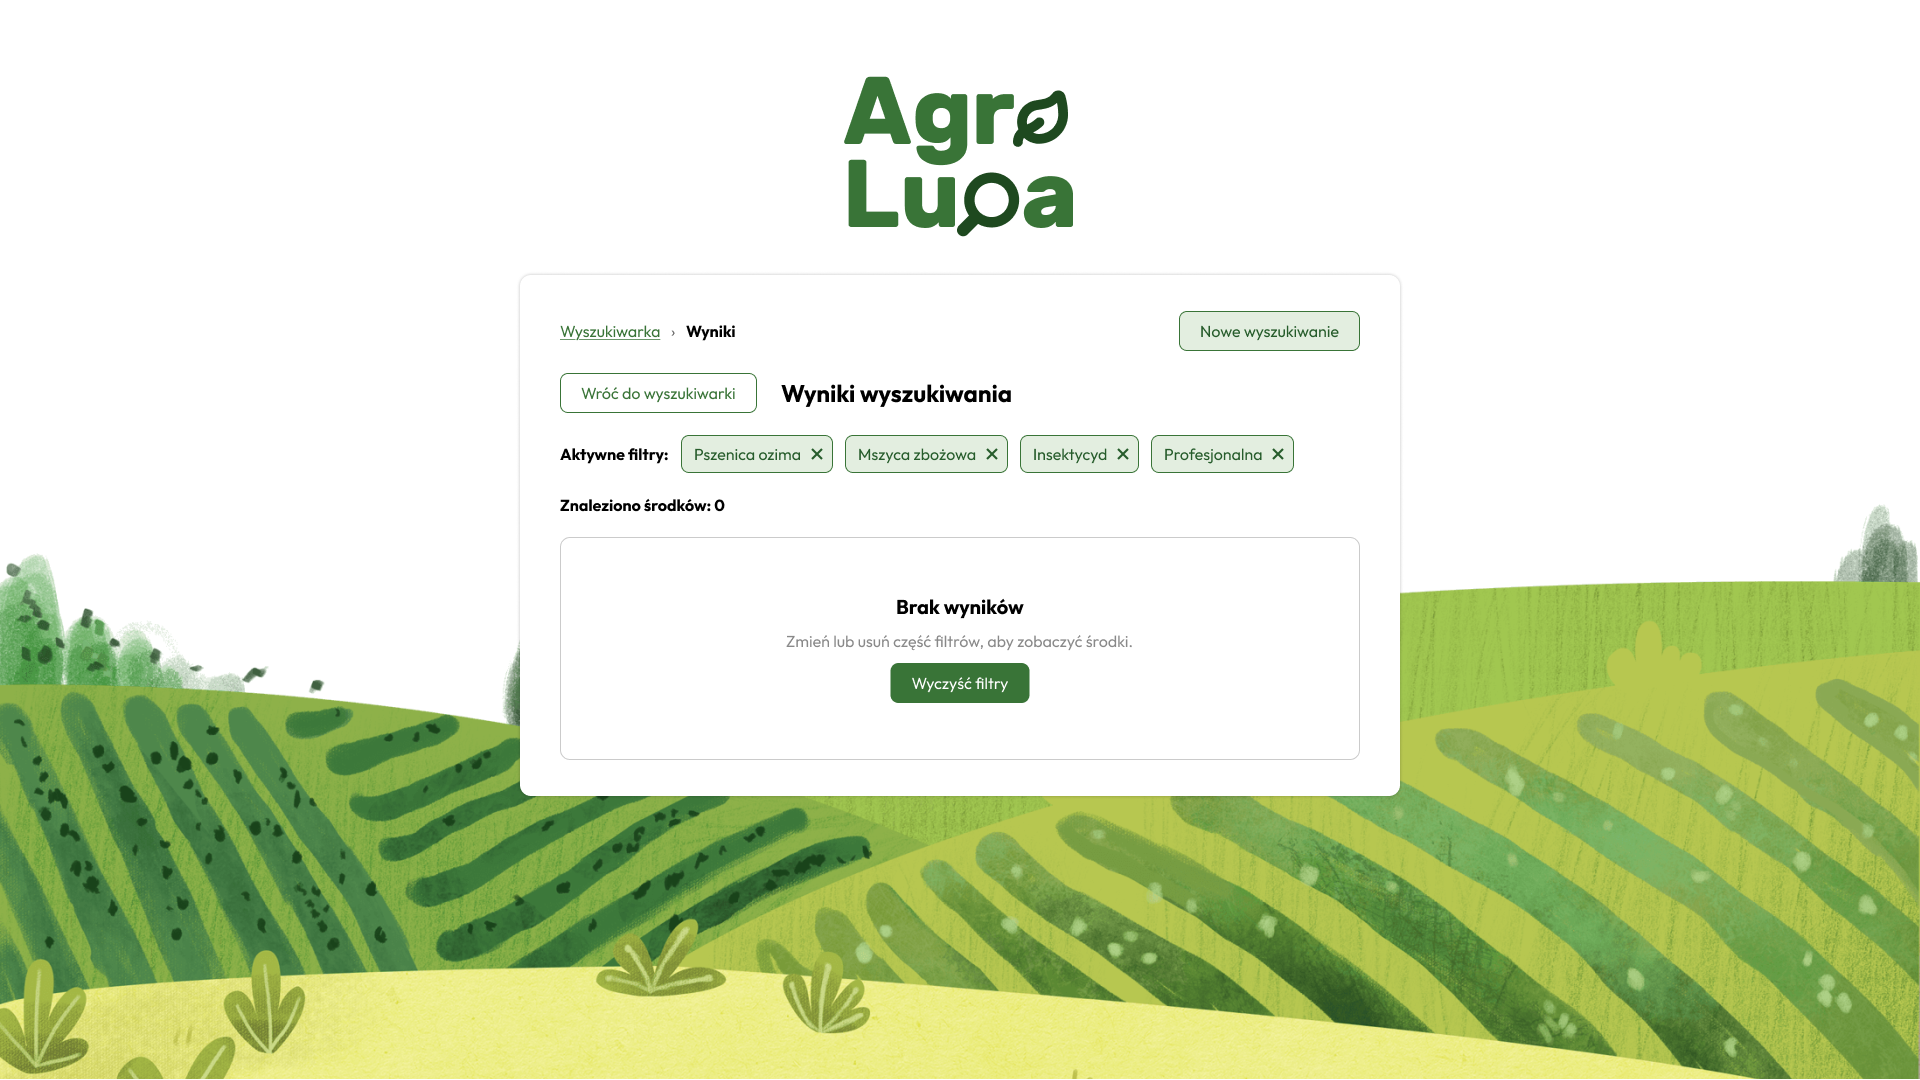
\includegraphics[width=\linewidth]{E-2_Lista_wynikow_brak_wynikow}
\end{center}

\subsubsection{E-3: Karta środka}

\begin{center}
    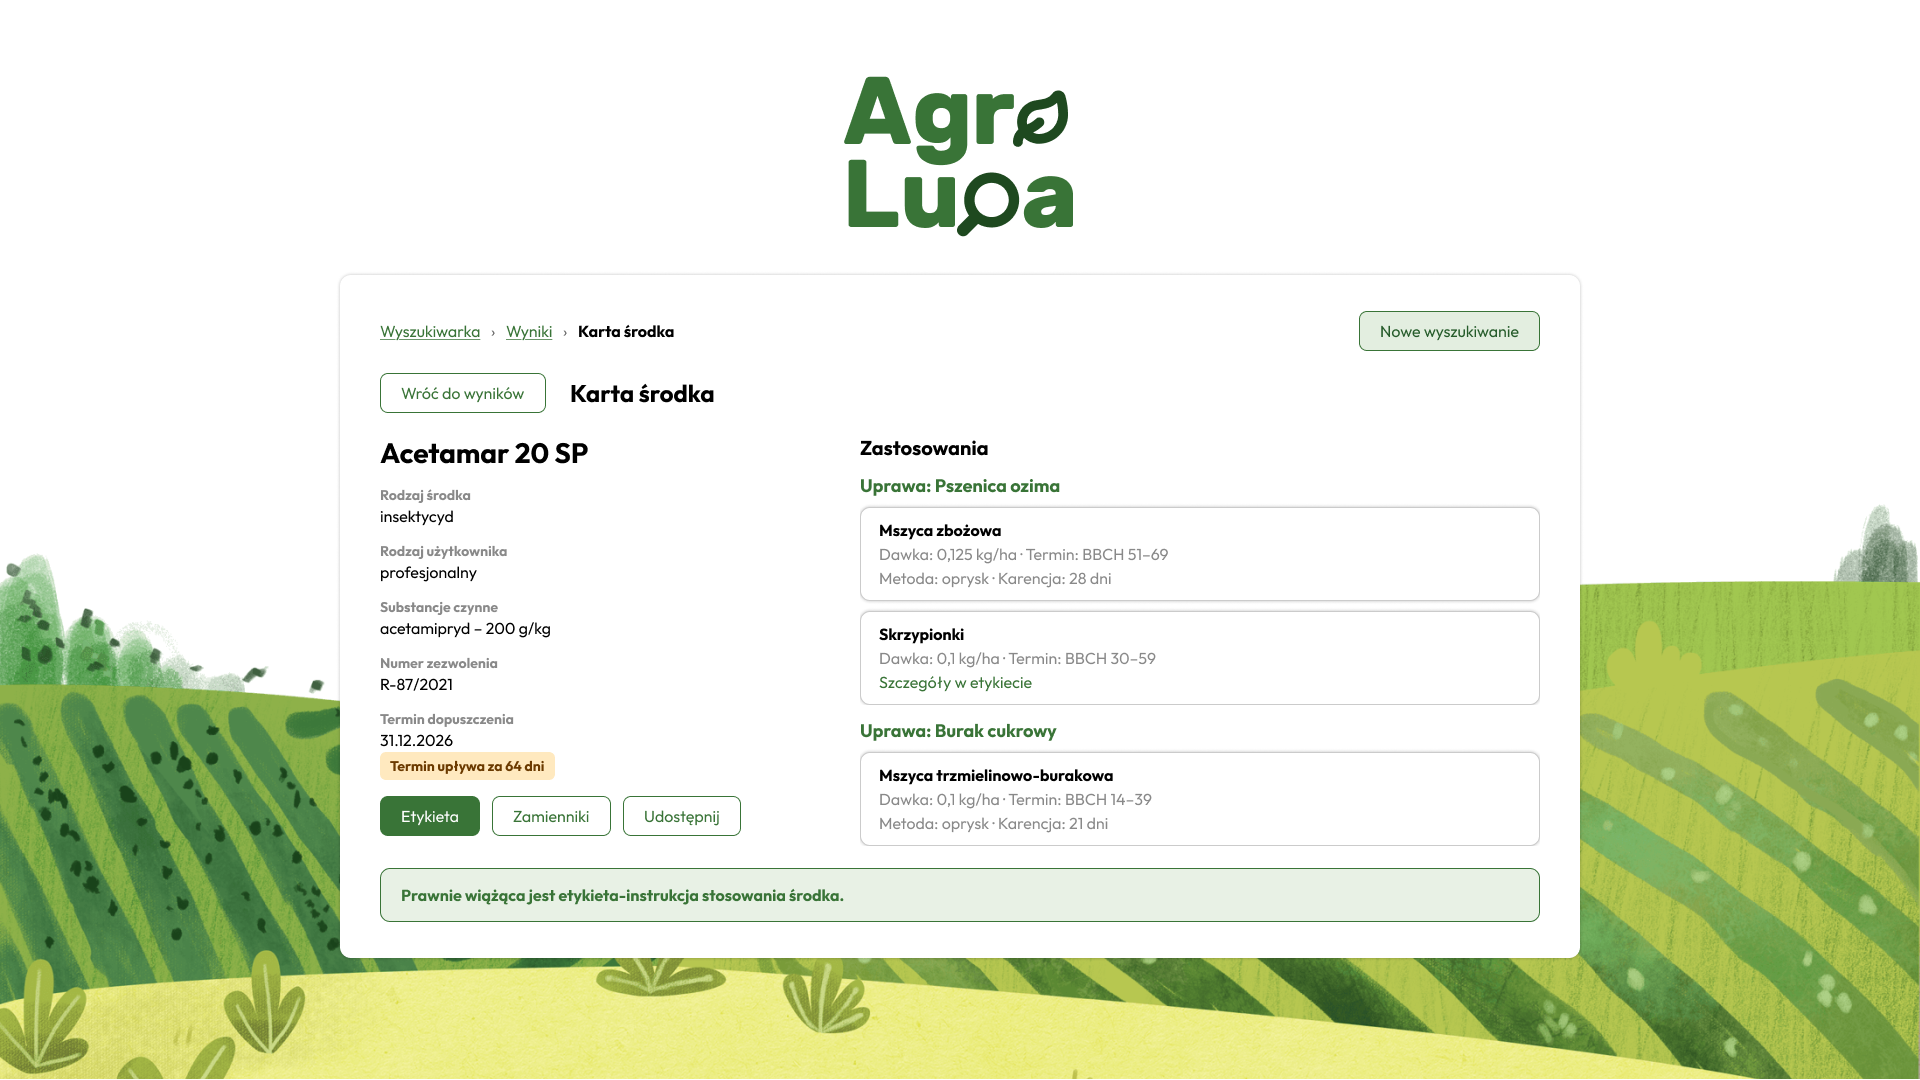
\includegraphics[width=\linewidth]{E-3_Karta_srodka}
\end{center}

\begin{itemize}
    \item dane środka zgodnie z~WF-06 oraz terminy z~oznaczeniem upływającego
    terminu (WF-11),
    \item lista zastosowań pogrupowana według upraw: agrofag, dawka, termin,
    metoda stosowania i~okres karencji lub odnośnik do etykiety (WF-07),
    \item przyciski: ,,Etykieta'', ,,Zamienniki'', ,,Udostępnij'' (WF-09,
    WF-10, WF-16),
    \item stała informacja, że prawnie wiążąca jest etykieta-instrukcja
    stosowania środka (O-02).
\end{itemize}

\subsubsection{E-4: Zamienniki}

\begin{center}
    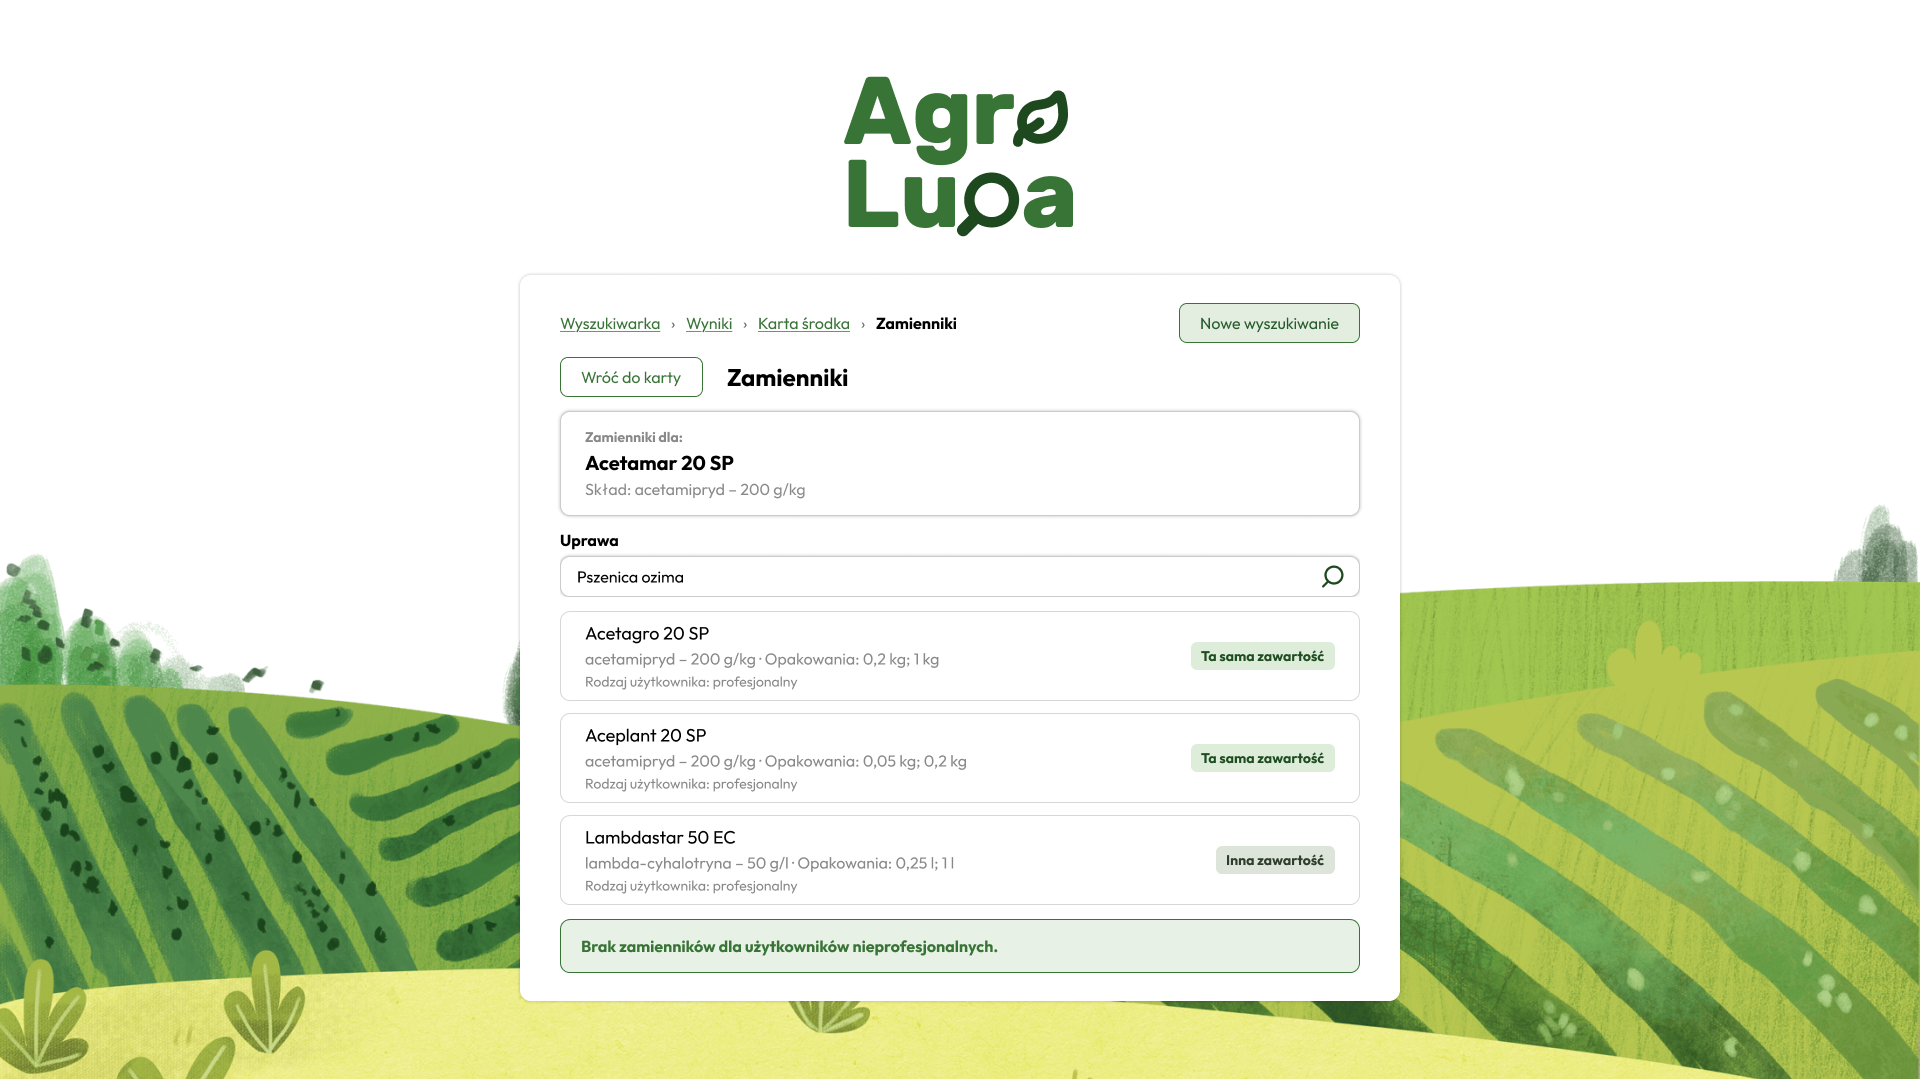
\includegraphics[width=\linewidth]{E-4_Zamienniki}
\end{center}

\begin{itemize}
    \item nazwa i~skład środka, dla którego wyszukano zamienniki,
    \item filtr uprawy,
    \item lista zamienników z~zawartością substancji czynnej, opakowaniami
    i~rodzajem użytkownika; środki o~tej samej zawartości na początku (WF-10),
    \item komunikat o~braku zamienników dla użytkowników nieprofesjonalnych.
\end{itemize}

\subsubsection{E-5: Podgląd etykiety}

\begin{center}
    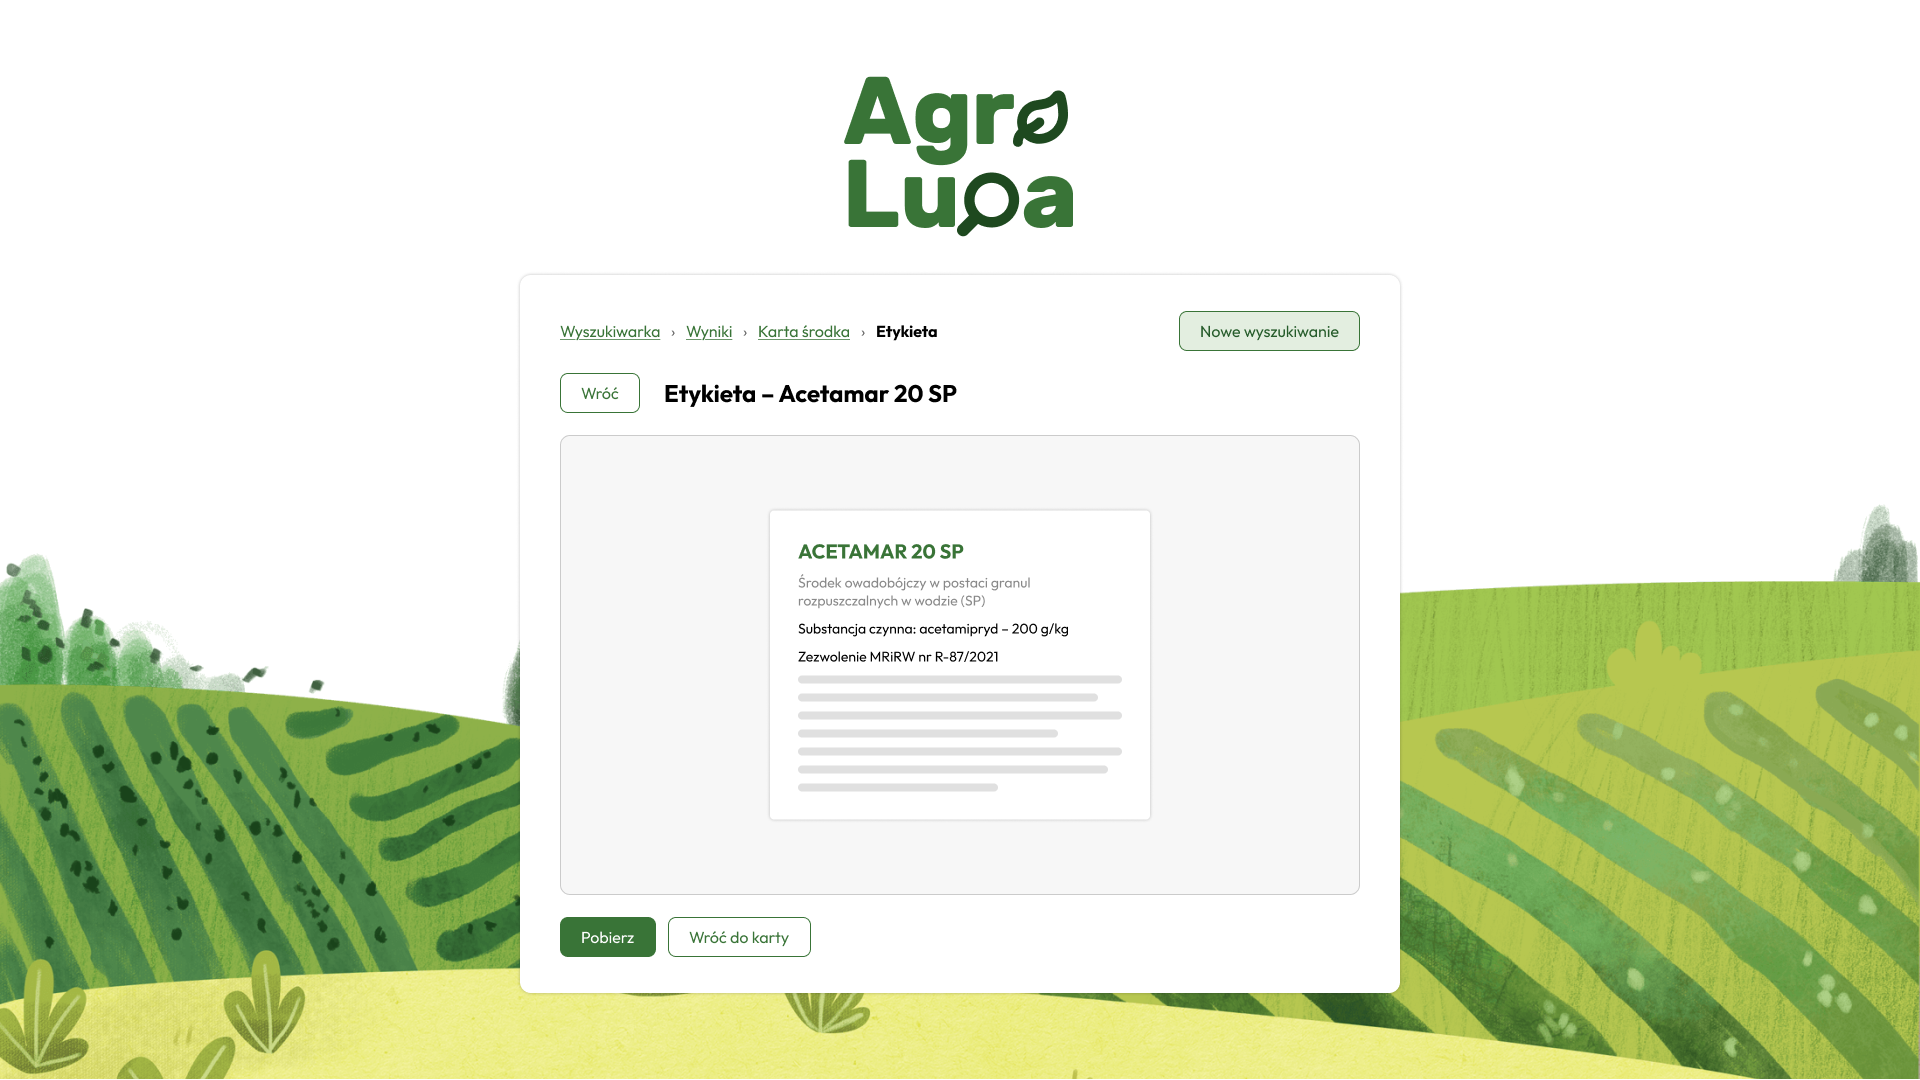
\includegraphics[width=\linewidth]{E-5_Podglad_etykiety}
\end{center}

\begin{itemize}
    \item etykieta wyświetlana w~aplikacji z~przyciskami ,,Pobierz''
    i~,,Wróć do karty'' (WF-09).
\end{itemize}

\subsection{Powiązanie z~wymaganiami}
\label{sec:powiazanie}

\begingroup
\small
\begin{longtable}{|p{1.7cm}|>{\raggedright\arraybackslash}p{2cm}|>{\raggedright\arraybackslash}p{3.3cm}|>{\raggedright\arraybackslash}p{1.6cm}|>{\raggedright\arraybackslash}p{5cm}|}
\hline
\textbf{Wymag.} & \textbf{Przypadek użycia} & \textbf{Moduł} & \textbf{Ekran} & \textbf{Dane i~inne elementy projektu} \\
\hline
\endfirsthead
\hline
\textbf{Wymag.} & \textbf{Przypadek użycia} & \textbf{Moduł} & \textbf{Ekran} & \textbf{Dane i~inne elementy projektu} \\
\hline
\endhead
WF-01 & PU-01 & Wyszukiwanie & E-1, E-2 & Środek \\
\hline
WF-02 & PU-01 -- PU-03 & Wyszukiwanie, Podpowiedzi & E-1 & indeksy trigramowe, pg\_trgm, fuzzystrmatch, unaccent \\
\hline
WF-03 & PU-02 & Wyszukiwanie & E-1, E-2 & Substancja czynna, Skład \\
\hline
WF-04 & PU-03 & Wyszukiwanie, Podpowiedzi & E-1, E-2 & Zastosowanie, Uprawa, Agrofag, Rodzaj środka \\
\hline
WF-05 & PU-03, PU-04, PU-07 & Wyszukiwanie, Zamienniki, Preferencje & E-1, E-2, E-4 & Środek: rodzaj użytkownika \\
\hline
WF-06 & PU-05 & Karta środka & E-3 & Środek, Skład, Zastosowanie \\
\hline
WF-07 & PU-05 & Karta środka & E-3 & Zastosowanie: okres karencji \\
\hline
WF-08 & PU-05 & Karta środka & E-3 & Zastosowanie: źródło okresu karencji \\
\hline
WF-09 & PU-06 & Etykiety & E-5 & Środek: odnośnik do etykiety \\
\hline
WF-10 & PU-07 & Zamienniki & E-4 & Skład: zawartość i~jednostka \\
\hline
WF-11 & PU-03, PU-05 & Karta środka & E-2, E-3 & Środek: terminy dopuszczenia \\
\hline
WF-12 & PU-01 & Wyszukiwanie & E-2 & Środek: data usunięcia z~rejestru \\
\hline
WF-13 & PU-10 & Import danych & -- & Import danych \\
\hline
WF-14 & PU-10 & Import danych & E-1 & Import danych: data publikacji \\
\hline
WF-15 & PU-08 & Preferencje & E-1 & pamięć przeglądarki \\
\hline
WF-16 & PU-09 & Karta środka & E-3 & stały adres oparty na id\_sor \\
\hline
WNF-01 & PU-01 -- PU-03 & Wyszukiwanie & -- & wyszukiwanie po stronie serwera, indeksy \\
\hline
WNF-02 & -- & Aplikacja kliencka & -- & przesyłanie wyłącznie wyników \\
\hline
WNF-03 --\newline WNF-05 &-- & Aplikacja kliencka & wszystkie & zasady projektowania ekranów \\
\hline
WNF-06 & -- & Aplikacja kliencka & wszystkie & aplikacja przeglądarkowa (O-03) \\
\hline
WNF-07 & PU-10 & Import danych & -- & codzienne sprawdzanie publikacji \\
\hline
WNF-08 & PU-10 & Import danych & -- & podmiana danych w~jednej transakcji, Import danych \\
\hline
WNF-09 & -- & -- & -- & brak uwierzytelniania, dane użytkownika w~przeglądarce \\
\hline
WNF-10 & -- & Aplikacja kliencka & wszystkie & nazewnictwo pól zgodne z~rejestrem \\
\hline
\end{longtable}
\endgroup
